% !TeX program = xelatex
\documentclass{nwputhesis}
\begin{document}

% 生成封面, 使用\maketitle
\maketitle

\newpage
% 中文摘要页
\makeabstract

听觉虚拟又可称为可听化,是近年来随着声学仿真技术的发展而出现的新概
念,即通过对包含单个(或多个)声源的声场进行物理或数学建模,以达到模拟
空间听音效果的目的。若考虑双耳效应,则可称为双耳听觉虚拟(Binaural 
Modeling)。

……

\myspace{1}% 空一行
 { \blackti 关键词:}听觉虚拟,HRTF,神经网络 

% 英文摘要页
\makeEnabstract

Virtual auditory technology is also called auralization. It is brought forward as a new concept with the development of acoustic simulation techniques in recent years and can be implemented by establishing the physical or mathematical models of a sound field to achieve sound effects simulation. If we consider the binaural effect, it can be called binaural virtual auditory.

……

\myspace{1}
 \textbf{ KEY WORDS:}virtual auditory, HRTF, neural network

% 目录
\makecontent

% 正文
\maketext

\section{绪论}
\subsection{可听化技术概述}
\subsubsection{可听化的概念}

可听化(Auralization)\upcite{bib:one}是近年来随着声学仿真技术的长足发展而出现的新概念,它的具体含义是通过对一包含单个(或者多个)声源的声场进行物理或数学建模,以达到声音绘制(Audio rendering)或称声学仿真(Acoustical simulation)的目的。这样,人们可以获得该声场中任意位置的双耳听觉感受。换句话说,可听化技术在客观上主要是模拟特定声场(包括声源、声传播环境以及聆听者三要素)中声音传播的物理过程,从而使其中的聆听者作为一个主体能够获得对整个场景声学特性的主观感知\upcite{bib:two,bib:three}。

\section{公式、表、图}
\subsection{公式}
\subsubsection{简单公式}
\begin{equation}
  \int_a^b f(x)\mathrm{d}x=F(b)-F(a)
\end{equation}

\subsubsection{多行公式}
如公式(\ref{q1})所示。
\begin{equation}
\label{q1}
\begin{aligned}
dx&=v_{x}dt\\
 dy&=v_{y}dt\\
x_{t+1}&=dx+x_{t}\\
y_{t+1}&=dx+y_{t}
\end{aligned}
\end{equation}

\subsubsection{括号公式}
如公式(\ref{q1})所示。
\begin{equation}
\left\{
\begin{aligned}
 100(t-kT_{2})   & , & t\in (kT_{2}, kT_{2}+0.2 )\\
20&,  & t\in (kT_{2}+0.2,kT_{2}+2.2)\\
-100t+240  & , & t\in( kT_{2}+2.2, kT_{2}+2.4)\\
0&,  & t\in (kT_{2}+2.4,(k+1)T_{2})
\end{aligned}
\right.
\end{equation}

\subsection{表格}
\subsubsection{简单表格}
如表\ref{table1}所示。

\begin{table}[H]
\fontsize{10.5bp}{1.25}
\caption{表格标题}
% \setlength{\abovecaptionskip}{0.2cm}  %调整标题与图距离
% \setlength{\belowcaptionskip}{0.2cm} %调整标题与下文距离
\centering\label{table1} 
% \vspace{-0.5em}	
\begin{tabular}{|c|c|c|c|}	
\hline % \toprule[1.5pt]
    方法 & A算法 & B算法 & C算法 \\ \hline
    误差/dB & 0.86 & 1.02 & 0.69 \\ \hline
    计算时间/s & 25 & 25 & 27 \\ \hline
\end{tabular}
\end{table}

\subsubsection{三线表}
三线表参考表\ref{table3}
\begin{table}[H]
\fontsize{10.5bp}{1.25}
\caption{表格标题}
% \setlength{\abovecaptionskip}{0.2cm}  %调整标题与图距离
% \setlength{\belowcaptionskip}{0.2cm} %调整标题与下文距离
\centering\label{table3} 
% \vspace{-0.5em}	
\begin{tabular}{cccc}	
\toprule[1.5pt]
    方法 & A算法 & B算法 & C算法 \\ 
    \toprule[1.5pt]
    误差/dB & 0.86 & 1.02 & 0.69 \\ 
    计算时间/s & 25 & 25 & 27 \\ 
    \toprule[1.5pt]
\end{tabular}
\end{table}

\subsubsection{精排表格}
较为复杂的表格参考表\ref{table2}
\begin{table}[H]
\caption{表格标题}
% \setlength{\abovecaptionskip}{0.2cm}  %调整标题与图距离
% \setlength{\belowcaptionskip}{-0.2cm} %调整标题与下文距离
\fontsize{10.5bp}{1.25}
\centering\label{table2} 
% \vspace{-0.5em}	
\begin{tabular}{|c|c|c|c|}	
\hline % \toprule[1.5pt]
\makecell*[c]{ Parameter Group \\ Condition Selection } &\makecell*[c]{ Basic Ways \\of Hatching  } 	& \makecell*[c]{Calculated Average\\ Alapsed Time} & \makecell*[c]{Calculated Average\\ Alapsed Time}  \\
\hline
\makecell*[c]{ Parameter group (1)\\ \\Parameter group (2)\\} &\makecell*[c]{ Zigzag   Hatch\\Contour Hatch\\Zigzag   Hatch\\Contour Hatch}& \makecell*[c]{468.940\\374.923 \\885.792\\1947.77}   & \makecell*[c]{Zigzag 1.888 \\ Contour  5.195   }   \\
\hline
\makecell*[c]{ Parameter group (1)\\ \\ Parameter group (2)\\}  &\makecell*[c]{ Zigzag   Hatch\\Contour Hatch\\Zigzag   Hatch\\Contour Hatch}&\makecell*[c]{ 545.080\\356.847\\1068.275\\1692.098} & \makecell*[c]{Zigzag 1.960 \\ Contour 4.742  }  \\
\hline
\end{tabular}
% \vspace{-1.5em}
\end{table}

\subsection{图片}
\subsubsection{单个图片}
单图如图\ref{P1}所示。
\begin{figure}[!ht]
\centering
%\vspace{-0.30cm} %设置与上面正文的距离`
%\setlength{\abovecaptionskip}{0.0cm}   %调整图片标题与图距离`
%\setlength{\belowcaptionskip}{0.0cm} %调整图片标题与下文距离
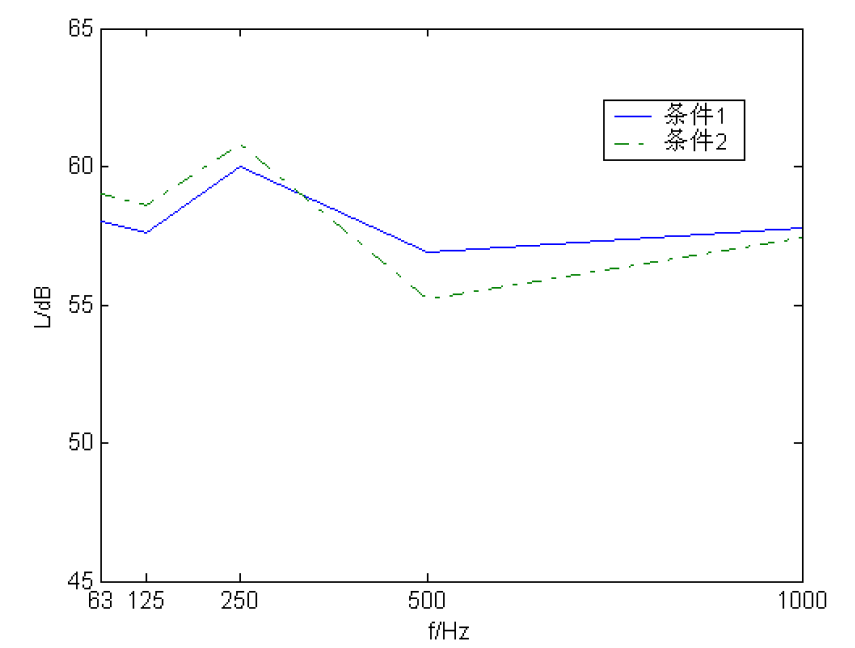
\includegraphics[width=4cm]{./picture/test.png}
\caption{图片标题}\label{P1}
\end{figure}
\subsubsection{子图}
多子图如图\ref{P2}、\ref{P2.1}、\ref{P2.2}所示。
\begin{figure}[h!]
  \centering
  \begin{subfigure}[b]{0.25\linewidth}
    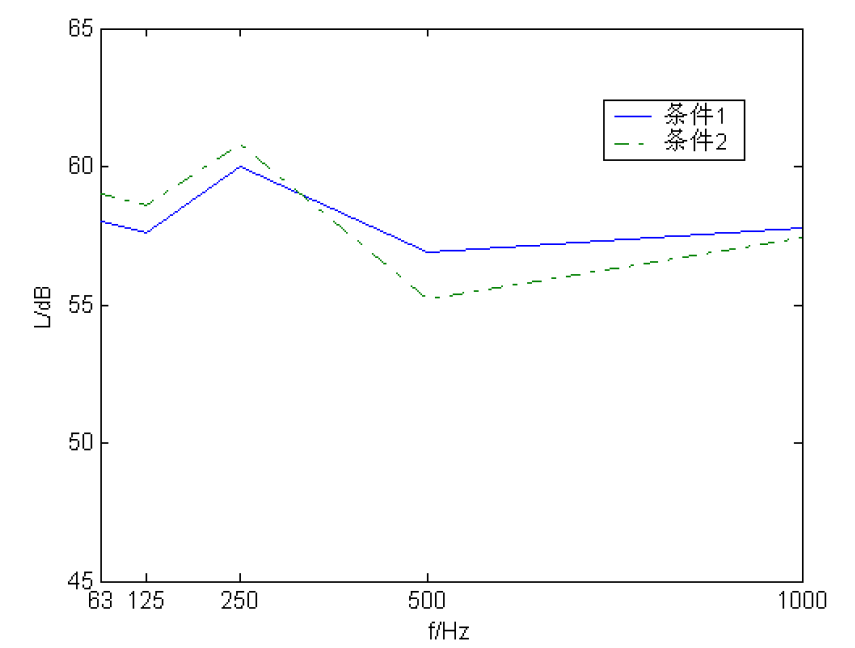
\includegraphics[width=\linewidth]{picture/test.png}
    \caption{图片标题1}\label{P2.1}
  \end{subfigure}
  \begin{subfigure}[b]{0.25\linewidth}
    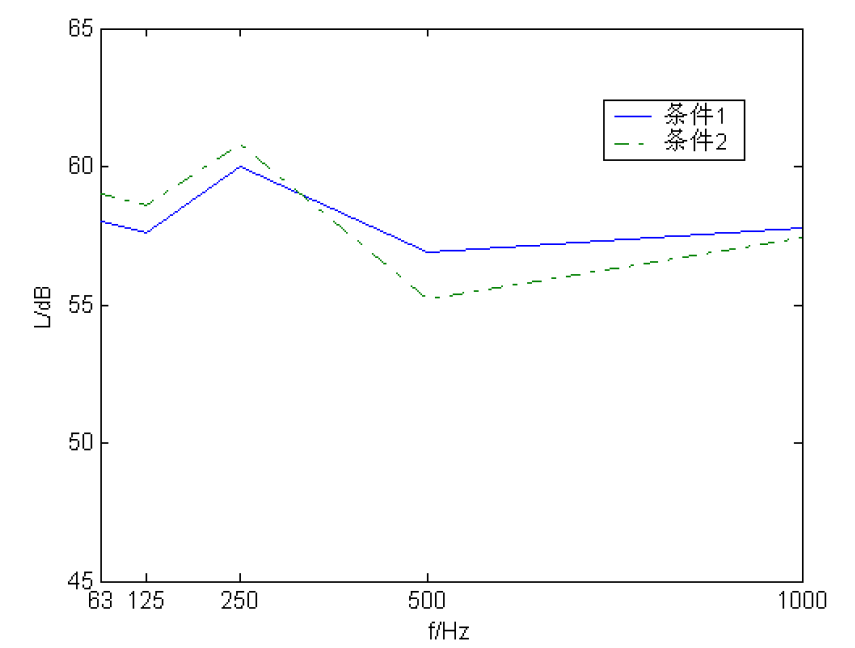
\includegraphics[width=\linewidth]{picture/test.png}
    \caption{图片标题2}\label{P2.2}
  \end{subfigure}
  \caption{总标题}
  \label{P2}
\end{figure}

% 参考文献
\newpage
\textcolor{white}{1}
\section*{参考文献}
\begingroup  % 去掉thebibliography环境自带的“参考文献”标题
\renewcommand{\section}[2]{} 
\addcontentsline{toc}{section}{参考文献}
\begin{thebibliography}{99}

\bibitem{bib:one}作者.题名[D].保存城市名:保存单位(写到二级单位),出版年.

\bibitem{bib:two}作者.题名[J].刊名,出版年,卷(期):起止页码..

\bibitem{bib:three}作者.题名[A].见[In];编者.论文集名[C].出版地:出版者,出版年.起止页码.
\iffalse
① 期刊    作者.题名[J].刊名,出版年,卷(期):起止页码.
② 论文集    作者.题名[A].见[In];编者.论文集名[C].出版地:出版者,出版年.起止页码.
③ 专著   作者.书名[M].版本(第1版免著).出版地:出版者,出版年.起止页码.
④ 学位论文    作者.题名[D].保存城市名:保存单位(写到二级单位),出版年.
⑤ 标准   起草责任者.标准代号标准顺序号-发布年,标准名称[S].出版地:出版者,出版年.
⑥ 科技报告     作者.题名[R].报告题名及编号,出版地:出版者,出版年.(起止页码).
⑦ 专利   专利所有者.题名  [P].专利国别:专利号,公告日期.
⑧ 电子文献   作者.题名.发表或更新日期/引用日期.电子文献地址.  
文献作者3名以内全部列出,4名以上只列出前3名,后加“,等”;
外文作者姓在前,首字为大写,名缩写为首字母,与姓之间空一字符,不加缩写点。
\fi
\end{thebibliography}

% 致谢
\section*{致谢}
\makespace %另起一页空两行
\begin{center}
    { \blackti \fontsize{16.0600pt}{1.25}致 \, 谢}
\end{center}
\addcontentsline{toc}{section}{致\textcolor{white}{1}谢}
\myspace{1}
致谢内容。

% 毕业设计小结
\section*{毕业设计小结}
\makespace
\begin{center}
    { \blackti \fontsize{16.0600pt}{1.25}毕业设计小结}
\end{center}
\addcontentsline{toc}{section}{毕业设计小结}
\myspace{1}
小结内容。

% 附录
\newpage
\section*{附录}
\makespace
\begin{center}
    { \blackti \fontsize{16.0600pt}{1.25}附\,录}
\end{center}
\addcontentsline{toc}{section}{附\textcolor{white}{1}录}
\myspace{1}
附录内容。
\end{document}

